\documentclass[pdflatex,sn-mathphys-num]{sn-jnl}

%%%% Standard Packages
\usepackage{graphicx}
\usepackage{multirow}
\usepackage{amsmath,amssymb,amsfonts}
\usepackage{amsthm}
\usepackage{mathrsfs}
\usepackage[title]{appendix}
\usepackage{xcolor}
\usepackage{textcomp}
\usepackage{manyfoot}
\usepackage{booktabs}
\usepackage{algorithm}
\usepackage{algorithmicx}
\usepackage{algpseudocode}
\usepackage{listings}
\usepackage{url}
\usepackage{lineno}
%%%%

%% Theorem Styles
\theoremstyle{thmstyleone}
\newtheorem{theorem}{Theorem}
\newtheorem{proposition}[theorem]{Proposition}

\theoremstyle{thmstyletwo}
\newtheorem{example}{Example}
\newtheorem{remark}{Remark}

\theoremstyle{thmstylethree}
\newtheorem{definition}{Definition}

%% Author-action marker. These flag unfinished author tasks that a writing
%% revision cannot complete. Strip them before submission (see
%% changes_2026-10-14.md, class C).

%% Hyphenation exceptions: 'ligand' must never break as 'lig-and',
%% which renders as a spurious repeated 'and' when followed by the word 'and'.
\hyphenation{li-gand nu-cle-ic}

\raggedbottom

\begin{document}

\linenumbers

\title[Bridging protein and nucleic-acid pockets]{Bridging protein and nucleic-acid pockets via shared physicochemical representations for 3D molecular generation with NA2smol}

\author[1]{\fnm{Letian} \sur{Gao}}
\author[2,7]{\fnm{Yi} \sur{Li}}
\author[1]{\fnm{Wenbiao} \sur{Zhou}}
\author[3]{\fnm{Jiahao} \sur{Chen}}
\author[2,8]{\fnm{Wenjin} \sur{Wan}}\email{wanwenjin@him.cas.cn}
\author[7]{\fnm{Yuxuan} \sur{Mo}}\email{moyuxuan25@mails.ucas.ac.cn}
\author*[4,5,6]{\fnm{Bing} \sur{Su}}\email{subingats@gmail.com}
\author*[2]{\fnm{Xing} \sur{Li}}\email{li@ioz.ac.cn}
\author*[1]{\fnm{Zhi John} \sur{Lu}}\email{zhilu@tsinghua.edu.cn}

\affil[1]{\orgname{MOE Key Laboratory of Bioinformatics, State Key Laboratory of Green Biomanufacturing, Center for Synthetic and Systems Biology, School of Life Sciences, Tsinghua University}, \orgaddress{\city{Beijing}, \country{China}}}
\affil[2]{\orgname{Interdisciplinary Science Center, State Key Laboratory of Animal Biodiversity Conservation and Integrated Pest Management, Institute of Zoology, Chinese Academy of Sciences}, \orgaddress{\street{No.1 West Beichen Road, Chaoyang District}, \city{Beijing} \postcode{100101}, \country{China}}}
\affil[3]{\orgname{Department of Automation, Tsinghua University}, \orgaddress{\city{Beijing}, \country{China}}}
\affil[4]{\orgname{Gaoling School of Artificial Intelligence, Renmin University of China}, \orgaddress{\city{Beijing}, \country{China}}}
\affil[5]{\orgname{Beijing Key Laboratory of Research on Large Models and Intelligent Governance}, \orgaddress{\city{Beijing}, \country{China}}}
\affil[6]{\orgname{Engineering Research Center of Next-Generation Intelligent Search and Recommendation, Ministry of Education}, \orgaddress{\city{Beijing}, \country{China}}}
\affil[7]{\orgname{University of Chinese Academy of Sciences}, \orgaddress{\city{Beijing} \postcode{100049}, \country{China}}}
\affil[8]{\orgname{Hangzhou Institute of Medicine, Chinese Academy of Sciences}, \orgaddress{\city{Hangzhou}, \postcode{310022}, \country{China}}}
\affil[]{These authors contributed equally: Letian Gao, Yi Li, Wenbiao Zhou and Jiahao Chen}
\affil[]{ORCID: Wenjin Wan, 0009-0008-4628-528X; Yuxuan Mo, 0009-0001-8521-845X}

\abstract{Three-dimensional molecular generation offers a route to designing compounds for nucleic-acid binding sites. Here we present NA2smol, a Bayesian flow network that generates molecules from nucleic-acid pockets using shared physicochemical descriptors, simulated electron-density pretraining and a teacher--student alignment loss. On an RNA test set, NA2smol achieved the highest multi-objective screening retention and reference-ligand recovery among six external generators. In a case study on the Clivia fluorogenic aptamer, the most frequently generated scaffold defined a combinatorial library whose members displaced the aptamer dye in solution and in cells, with half-maximal inhibitory concentrations of 3.3 and 3.2~$\mu$M. In a final case study on the KRAS promoter G-quadruplex, generation followed by post-processing prioritised a bis-benzothiazole that reduced normalised thioflavin T (ThT) fluorescence in a concentration-dependent manner, with an apparent half-maximal concentration (DC$_{50}$) of 22.4~$\mu$M. NA2smol provides a framework for pocket-conditioned molecular design against nucleic acids and computational prioritisation for experimental follow-up.}

\keywords{molecular generation, deep learning, nucleic-acid ligand, Bayesian flow network, transfer learning}

\maketitle

Structure-based molecular generation aims to produce chemically plausible ligand candidates directly from three-dimensional target structures. For protein pockets, pocket-conditioned generators propose molecules with favourable docking scores and drug-like properties \cite{pocket2mol2022,targetdiff2023,diffsbdd2024,molcraft2024}, density-based conditioning is an established alternative \cite{ed2mol2025,ecloudgen2025}, and flow matching and pocket-sequence conditioning are adjacent approaches \cite{flowr2026,pockliggpt2026}. Nucleic acids are an important therapeutic target class, with small molecules able to modulate splicing, translation, riboswitches, non-coding RNA function, RNA--protein interactions and structured DNA/RNA motifs \cite{childsdisney2022rna,g4ldb2025}, yet their pockets remain underrepresented in molecular generation. Existing computational work falls into three categories \cite{rnamigos2025,smrtnet2026,ribostrike2024,karroucha2025rnaml}: two predict RNA--ligand interactions or rank an existing library against a fixed structure, while the third generates structures directly, and this generative category is the least developed. Recent RNA-pocket methods identify potential binding sites rather than generate ligands conditioned on an explicitly supplied pocket \cite{smartpocket2026,ribolens2026}. To our knowledge, three-dimensional ligand structures have not previously been generated directly from the geometry and physicochemical environment of an explicitly supplied nucleic-acid binding pocket.

The primary bottleneck is the scarcity of nucleic-acid--small-molecule complex structures. Protein training draws on experimentally resolved complexes in the Protein Data Bank \cite{berman2000pdb} and on millions of docked poses \cite{francoeur2020crossdocked}, whereas curated nucleic-acid--ligand resources contain hundreds of non-redundant entries; the set assembled here comprises 738 complex records (457 RNA, 274 DNA and 7 hybrid) \cite{hariboss2022,rnamigos2025,smrtnet2026,g4ldb2025}. Pocket representation is a second barrier: most pocket-conditioned generators use amino-acid-specific residue features, which have no nucleotide analogue and motivate a representation applicable to both classes of pocket.

Protein and nucleic-acid pockets differ in composition and structural organisation, but both present physicochemical environments that constrain ligand compatibility, motivating a representation of local pocket environments through shared physicochemical features. We designed NA2smol, a Bayesian flow network (BFN) generator \cite{graves2023bfn} built around two design choices (Fig.~1). The first is a shared pocket representation restricted to descriptors common to both classes: pharmacophore type, hybridisation state, van der Waals radius and partial charge. The second couples an electron-density (ED) encoder and a pocket encoder to a shared molecular generator. Ligand-only simulated electron-density pretraining \cite{ed2mol2025} provides structural supervision from pharmacophore-labelled density maps, a training-time constraint aligns the pocket-conditioned student with a frozen pretrained ED-conditioned teacher, and fine-tuning uses protein--ligand and nucleic-acid--ligand complexes. The candidate library can be post-processed for a specific application (Fig.~1, right).

We evaluate generated molecules on an RNA test set assembled with the SMRTnet method \cite{smrtnet2026} using target-level reference recovery and a multi-objective screening cascade, and assess protein-benchmark behaviour on the Directory of Useful Decoys, Enhanced (DUD-E) \cite{dude2012} under the same pipeline while comparing training configurations. We then apply the generator to the Clivia fluorogenic aptamer and test members of the resulting combinatorial library in competition and cellular assays, and finally post-process a generated library to prioritise candidates for the KRAS promoter G-quadruplex and test one compound in a ThT displacement assay.

\begin{figure}[!htbp]
\centering
\centerline{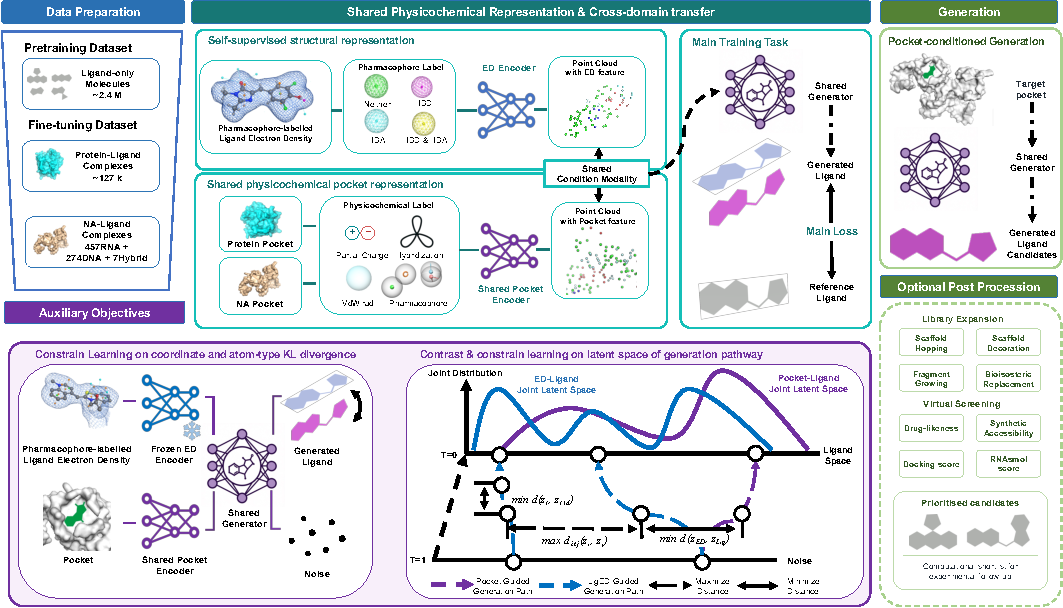
\includegraphics[width=180mm]{figures/figure1_nbt.pdf}}
\caption{Workflow, training and candidate-prioritisation strategy of NA2smol. \textbf{Data preparation} (top left). Pretraining uses a ligand-only library ($\sim$2.4~M molecules) represented as pharmacophore-labelled ligand ED maps. Fine-tuning uses protein--ligand ($\sim$127~k) and nucleic-acid--ligand complexes (738 curated records: 356 training and 382 validation; Supplementary Tables~5 and~9). \textbf{Shared physicochemical representation and cross-domain transfer} (top centre). A self-supervised encoder maps four-class pharmacophore-labelled ligand ED (neither, HBD only, HBA only, or both) to an ED point cloud. In parallel, a shared pocket encoder maps protein or nucleic-acid pockets to a physicochemical point cloud (partial charge, hybridisation, van der Waals radii and pharmacophore label) feeding the shared generator (Methods). \textbf{Auxiliary objectives} (bottom left). Constrained learning on the predicted outputs aligns the pocket-conditioned student with the frozen ED teacher on coordinates and atom-type distributions. Contrastive learning acts on flow states during ED pretraining ($d(z_i,z_{i+\Delta})$ and $d_{\mathrm{iff}}(z_i,z_j)$) and across teacher and student views for the full model during fine-tuning ($d(z_{\mathrm{ED}},z_{\mathrm{lig}})$). \textbf{Generation} (top right). Conditioned on a target pocket, the shared generator produces candidate ligands. \textbf{Optional post-processing} (right). Candidates can undergo library expansion and multi-objective virtual screening (drug-likeness, synthetic accessibility, docking score and RNAsmol score) to prioritise compounds for experimental follow-up. Schematic time $T$ runs opposite to sampling time $t$ in Methods ($T=1-t$). LigED, ligand electron density; NA, nucleic acid; HBD and HBA, hydrogen-bond donor and acceptor; VdW, van der Waals.}
\label{overview}
\end{figure}

\section{Results}\label{sec2}

\subsection{Experimental design}

NA2smol is a BFN generator conditioned on transferable physicochemical features (pharmacophore labels, hybridisation states, van der Waals radii and partial charges). Training has two stages: pretraining on ligand-only simulated electron-density maps yielding a frozen ED-conditioned teacher, and fine-tuning on protein--ligand and nucleic-acid--ligand complexes with the pocket-conditioned student aligned to that teacher.

Following the continuous-space design of MolCRAFT \cite{molcraft2024}, NA2smol progressively corrupts ligand states and reconstructs them conditional on both the noisy ligand and the pocket structure (Methods).

\subsection{Transferable pocket-conditioned generation on RNA and protein targets}

\begin{figure}[!htbp]
\centering
\makebox[\textwidth][c]{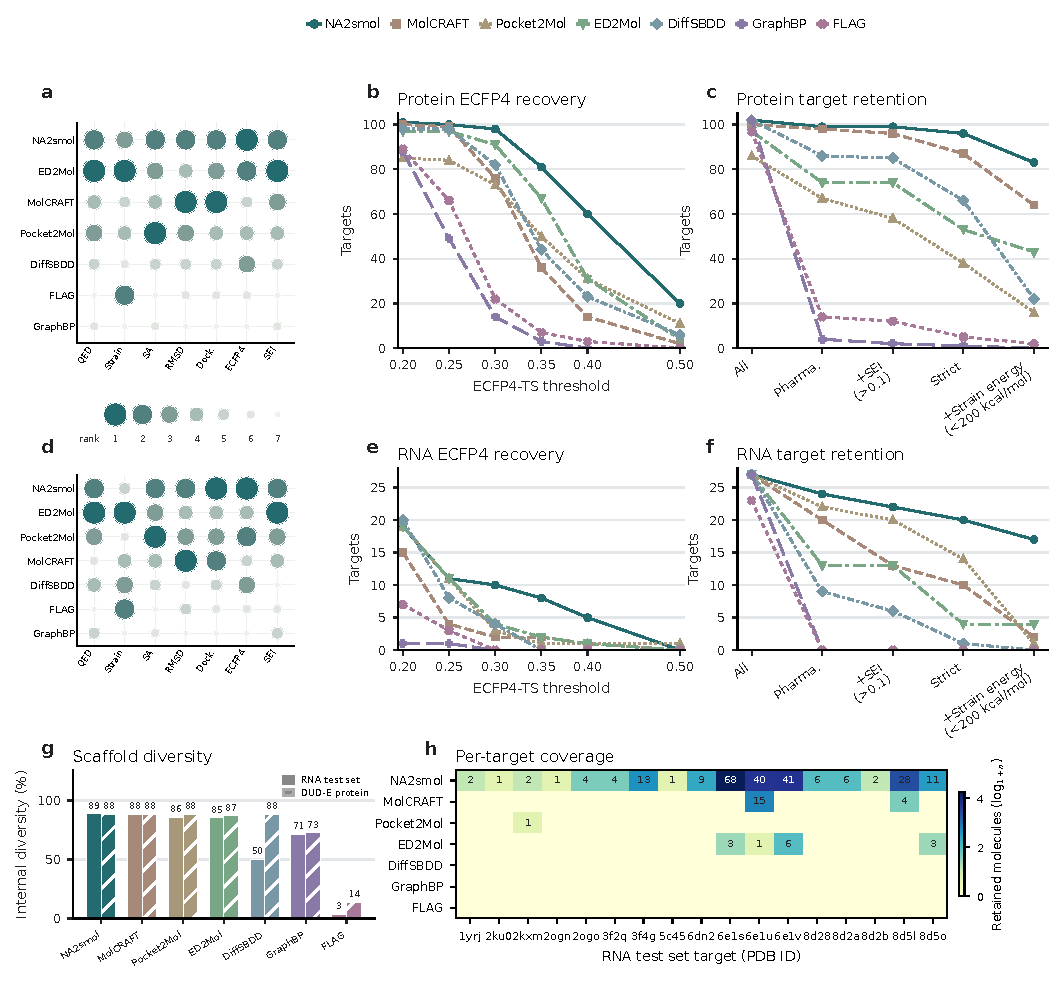
\includegraphics[width=180mm]{figures/figure2_nbt.pdf}}
\caption{Paired benchmark evaluation on the DUD-E protein benchmark and the RNA test set (27 shared evaluable RNA targets). a, DUD-E method-by-metric rank grid across seven axes (Dock., docking score; RMSD after pose relaxation; QED, quantitative estimate of drug-likeness; SA, synthetic accessibility score; SEI, surface efficiency index; ECFP4, extended-connectivity fingerprint similarity; and Strain, conformational strain energy). Bubble diameter and shade encode method rank on each axis from best (largest, darkest) to worst (smallest, palest) across NA2smol and six external generators (MolCRAFT, Pocket2Mol, ED2Mol, DiffSBDD, GraphBP and FLAG). Axis definitions are in Methods, raw medians in Table~1 and normalised scores in Extended Data Table~8. b, DUD-E reference-ligand recovery over the fixed 101-target reference universe; missing valid output counts as unrecovered, as on the ECFP4 axis in panel a. c, DUD-E screening retention as absolute target counts over method-specific outputs (85--102 targets per method) across the four-tier cascade (Methods). d, RNA test-set method-by-metric rank grid corresponding to panel a. e,f, RNA test-set reference-ligand recovery (e) and screening retention (f) across the 27 shared evaluable targets. g, Internal scaffold diversity: unique Bemis--Murcko \cite{bemis1996} scaffolds as a percentage of each method's distinct generated molecules (solid bars, RNA test set; hatched bars, DUD-E). h, Per-target candidate coverage under the most stringent filter on the RNA test set (retained molecule counts on a logarithmic colour scale).}
\label{benchmark_pair_fig}
\end{figure}

We evaluated the RNA test set and the DUD-E protein benchmark in parallel using the same metrics and screening logic (Fig.~2). The RNA test set comprises 37 RNA pocket--ligand systems; after validity filtering, 27 shared evaluable targets remained (the same set for every method, 1,000 molecules per pocket), and all valid molecules with negative docking scores entered the downstream evaluation. We compared NA2smol with six external structure-based generators, MolCRAFT, Pocket2Mol, ED2Mol, DiffSBDD \cite{diffsbdd2024}, GraphBP \cite{liu2023graphbp} and FLAG \cite{zhang2023flag}, each run with its published protein-oriented checkpoint under the same docking, filtering and evaluation pipeline (Methods).

In the RNA test set, NA2smol gave a more negative docking score, higher QED and LLE, and a lower SA score than the external generators, whereas pose-relaxation RMSD and surface efficiency index (SEI) were similar across methods (Fig.~2d); for NA2smol neither differed from its own baseline (two-sided Wilcoxon $P=1.00$ and $P=0.35$; Extended Data Table~3). In the DUD-E control it stayed within the range of the protein-trained baselines on docking, drug-likeness and strain (Fig.~2a), and under the most stringent filter it retained 3,726 molecules across 83 targets against 2,361 across 64 for the best baseline, MolCRAFT.

ECFP4 Tanimoto similarity (ECFP4-TS) to known RNA actives was summarised as target-level recovery (Methods, Eq.~10). Target recovery of NA2smol exceeded that of every protein-trained baseline across the whole threshold window (Fig.~2e). We also audited chemical overlap between benchmark actives and training ligands and tested the robustness of recovery to it (Methods; Supplementary Note~5).

Exact identity between generated molecules and fine-tuning ligands was rare on both benchmarks, whereas similarity to the ligand-only pretraining library was higher (Supplementary Table~5). Excluding exact fine-tuning matches changed recovery little, and removing targets whose actives resemble the fine-tuning partition left NA2smol ahead on both benchmarks. Removing targets whose actives resemble the pretraining library changed the ranking, with NA2smol falling below ED2Mol on RNA and DiffSBDD on DUD-E: recovery fell from 0.68 to 0.24 on DUD-E and from 0.218 to 0.053 on RNA. The full model showed the largest drop among the three pretrained configurations, $-0.198$ on the matched subset against $-0.099$ with alignment alone and $-0.014$ with pretraining alone (Fig.~3g; Extended Data Tables~6 and~7; Supplementary Note~5). Excluding actives by structure identifier rather than by record preserved the ranking direction (Supplementary Table~2).

Separation was largest under a four-tier virtual-screening cascade combining docking score, drug-likeness, synthetic accessibility, surface efficiency and conformational strain (thresholds in Methods; Fig.~2f): NA2smol retention was higher at every tier, in molecule counts and target coverage, and under the most stringent tier it retained 239 molecules across 17 of the 27 evaluable targets (0.68\% of 35,358 valid generations), with ten targets returning no molecule.



Single-metric strengths did not translate into multi-objective retention. MolCRAFT performed well on docking score and pose-relaxation RMSD, and ED2Mol on QED and strain, consistent with transferable steric priors and with fragment-based, density-conditioned construction; yet under the most stringent tier they retained 19 molecules across 2 targets and 13 across 4, respectively, and Pocket2Mol one molecule in one target.

After the +SEI gate, NA2smol spanned 5,671 unique Bemis--Murcko scaffolds \cite{bemis1996} on the RNA test set and 24,270 on DUD-E, 8.1-fold and 2.9-fold the largest baseline count (Pocket2Mol, 700; MolCRAFT, 8,316; Fig.~2g; Extended Data Table~2). At matched library size, the RNA advantage disappeared and the DUD-E advantage reversed (Supplementary Table~1). Raw scaffold counts therefore track screening yield rather than library-wide chemical diversity.

\subsection{The training components act on different candidate properties}

\begin{figure}[!htbp]
\centering
\makebox[\textwidth][c]{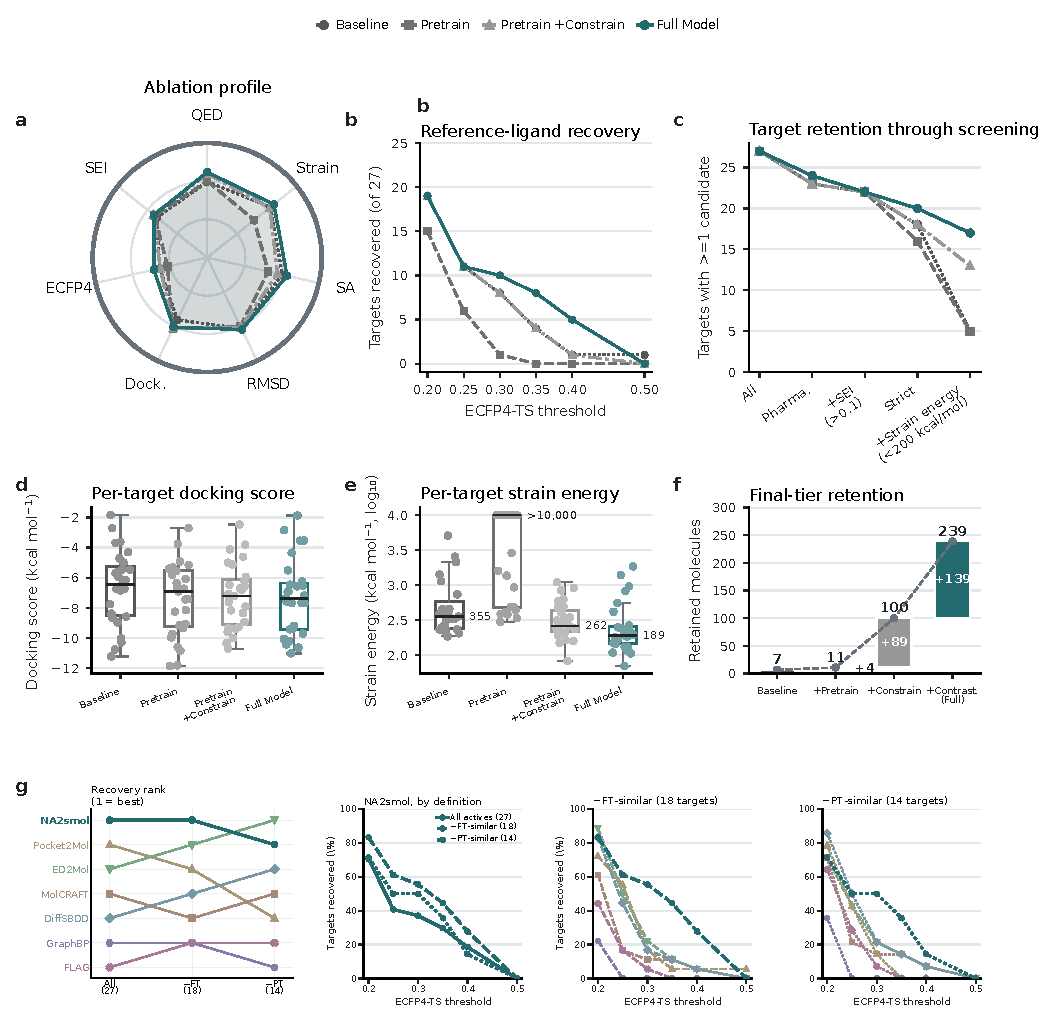
\includegraphics[width=180mm]{figures/figure3_nbt.pdf}}
\caption{Comparison of NA2smol training configurations on the RNA test set (four configurations, $n=27$ targets per configuration). a, Ablation profile across the same seven metrics as Fig.~2d (docking, RMSD, QED, SA, SEI and Strain as retention-curve integrals; ECFP4 recovery as its raw area); a larger radial distance means better performance. b, Reference-ligand recovery: targets with at least one molecule reaching the ECFP4-Tanimoto similarity threshold. c, Targets with at least one retained molecule through the screening cascade. d, Per-target smina docking-score distributions. e, Per-target conformational strain energy (PoseCheck \cite{harris2023posecheck}) on a $\log_{10}$ scale; labels give the median of per-target medians in kcal~mol$^{-1}$, with medians at the $10^{4}$ bound labelled $>10,000$. f, Differences in retained molecule counts between successive configurations (waterfall); bars show incremental gain and the dashed line the cumulative total. g, ECFP4 recovery across similarity-filtered target subsets (four panels): recovery rank of each method on the three target sets (all actives, 27; fine-tuning-similar actives removed, 18; pretraining-library-similar actives removed, 14), with method colours keyed on the left axis and vertical position giving the rank (1 = best); NA2smol recovery curves on the same three target sets; and recovery curves of all seven methods on the fine-tuning-similar-removed and pretraining-similar-removed subsets (fraction of eligible targets with at least one molecule above the ECFP4-Tanimoto similarity threshold; Extended Data Table~6). For e, strain values above $10^{4}$~kcal~mol$^{-1}$ and failed evaluations were set to $10^{4}$~kcal~mol$^{-1}$; in d,e, boxes show the interquartile range, centre lines medians and points target-level medians.}
\label{ablation_fig}
\end{figure}

We compared four configurations on the RNA test set, forming a ladder across the auxiliary objectives: the baseline uses the same architecture with only the primary Bayesian-flow losses active; Pretrain-Only starts from the pretrained weights without a teacher checkpoint, so neither alignment nor contrastive learning is applied; Pretrain+Constrain adds electron-density-teacher to pocket-student alignment; and the full model adds the cross-view contrastive loss on top of that alignment.

Pretrain-Only showed the largest change in docking score relative to the baseline (mean of per-target means, $-6.559$ to $-7.456$~kcal~mol$^{-1}$; Extended Data Table~3) but at a cost in conformational plausibility: its strain energies were far higher than those of the other configurations (Fig.~3e), with 48.5\% of molecules above the $10^{4}$~kcal~mol$^{-1}$ censoring bound, against none for ED2Mol and 7.7--14.9\% for the other configurations (Extended Data Table~4). The high strain was therefore widespread rather than outlier-driven. Pretrain+Constrain markedly reduced strain while largely retaining the docking gain, and SA score and QED recovered towards the full model (Fig.~3a).

Among the four configurations the full model had the most favourable multi-property profile (Fig.~3a). Final-tier retention rose from 7 molecules across 5 targets for the baseline to 11 across 5 for Pretrain-Only, 100 across 13 for Pretrain+Constrain and 239 across 17 for the full model (Fig.~3f; increments $+4$, $+89$ and $+139$ molecules).


\subsection{NA2smol generation defines a combinatorial library around the reproducible scaffold of the Clivia aptamer}

Fluorogenic RNA aptamers such as Clivia bind small-molecule dyes that become fluorescent in the bound state, making the dye-occupied site a defined pocket for structure-based design. We collected the seven Clivia structures in the Protein Data Bank (8HZD, 8HZE, 8HZF, 8HZJ, 8HZK, 8HZL and 8HZM), extracted a ligand-defined pocket around every crystallographically independent dye (18 pockets) and superposed them: 14 of the 16 comparable pockets form a single site (C4$'$/P RMSD 0.22--0.81~\AA, median 0.53~\AA) occupied by all four chemically distinct dyes (Fig.~4a). Generation used the representative 8HZE\_A109 pocket (23 nucleotides; Methods).

Conditioning NA2smol on this pocket produced 10,000 molecules in 100 sampling steps, and bond recovery with OpenBabel followed by valence and sanitisation filtering left 9,880 closed-shell, neutral molecules. A fluorogenic ligand requires an extended $\pi$-system, so we retained molecules whose largest sp$^{2}$-connected component spans at least 20 atoms (the value measured for all four Clivia crystal dyes, NI4, O2I, NJL and O00) with at least two aromatic rings, SA score $\leq 4$, molar mass 250--600~Da, TPSA $\leq 120$~\AA$^{2}$ and at most nine rotatable bonds (Fig.~4b). This left 996 molecules and 777 Bemis--Murcko scaffolds; most appeared once or twice, whereas the 2,4-diarylquinoline core appeared 15 times, more often than any other, and was taken as the design core (Fig.~4b).

Holding the ring system fixed and running inpainting produced 5,100 products, 4,948 of which retained the complete three-ring system. We recorded the substituent placed at each of the three variable positions: the para positions of the C4- and C2-aryl rings and the quinoline C7 position (Fig.~4c). H, OMe and OH dominated; OEt appeared mainly at C2 and C7, Cl at all three positions, and NMe$_{2}$, NHMe and NH$_{2}$ only rarely, while CN, COOH and CONH$_{2}$ were never produced. Enumerating all combinations placed at least once at each position gave 448 molecules (Fig.~4c).

Poses were scored by minimising each molecule in place with the rDock nucleic-acid scoring function under a rigid receptor, and the four crystal dyes were scored from their crystallographic coordinates after superposition on the 8HZE frame (pocket RMSD 0.42--0.56~\AA). The validated dye NI4 scores $-38.9$, better than 96\% of the 1,908 scored molecules, and all four dyes rank in the best quarter of the distribution (Fig.~4f). Drug-likeness gates (QED $\geq 0.44$, SA score $\leq 2.00$; Fig.~4e) left 198 candidates, ranked by the mean percentile of the minimised rDock and SA scores. Both reference compounds are in this library, at ranks 43 (Al-1) and 67 (Al-2), and both occupy the same pocket site (Fig.~4d).

We tested both compounds. In a competition assay against the Clivia dye, fluorescence decreased with concentration and fitted a four-parameter logistic model, giving Al-1 IC$_{50}$ $=3.29$~$\mu$M ($n=16$ wells) and Al-2 IC$_{50}$ $=3.16$~$\mu$M ($n=14$ wells; Fig.~4g); the two are equipotent (IC$_{50}$ ratio 0.96) and differ mainly in the lower plateau. In Clivia-expressing HEK293T cells (NBSI618 channel, Hoechst counterstain) fluorescence fell in every treatment group relative to untreated cells (Mock, 100\%): Al-1 to 43.4\% $\pm$ 2.1\% at 1~$\mu$M and 34.9\% $\pm$ 1.5\% at 10~$\mu$M, Al-2 to 73.7\% $\pm$ 2.4\% and 41.9\% $\pm$ 1.3\% (mean $\pm$ SEM over 93 cells per condition; Welch $t$-test versus Mock, Holm-corrected, all $P<10^{-4}$; Fig.~4h,i). A pocket-conditioned generative workflow recovered a scaffold the model reproduces, defined a synthesisable library around it and identified compounds that displace the dye in solution and in cells.

\begin{figure}[!htbp]
\centering
\makebox[\textwidth][c]{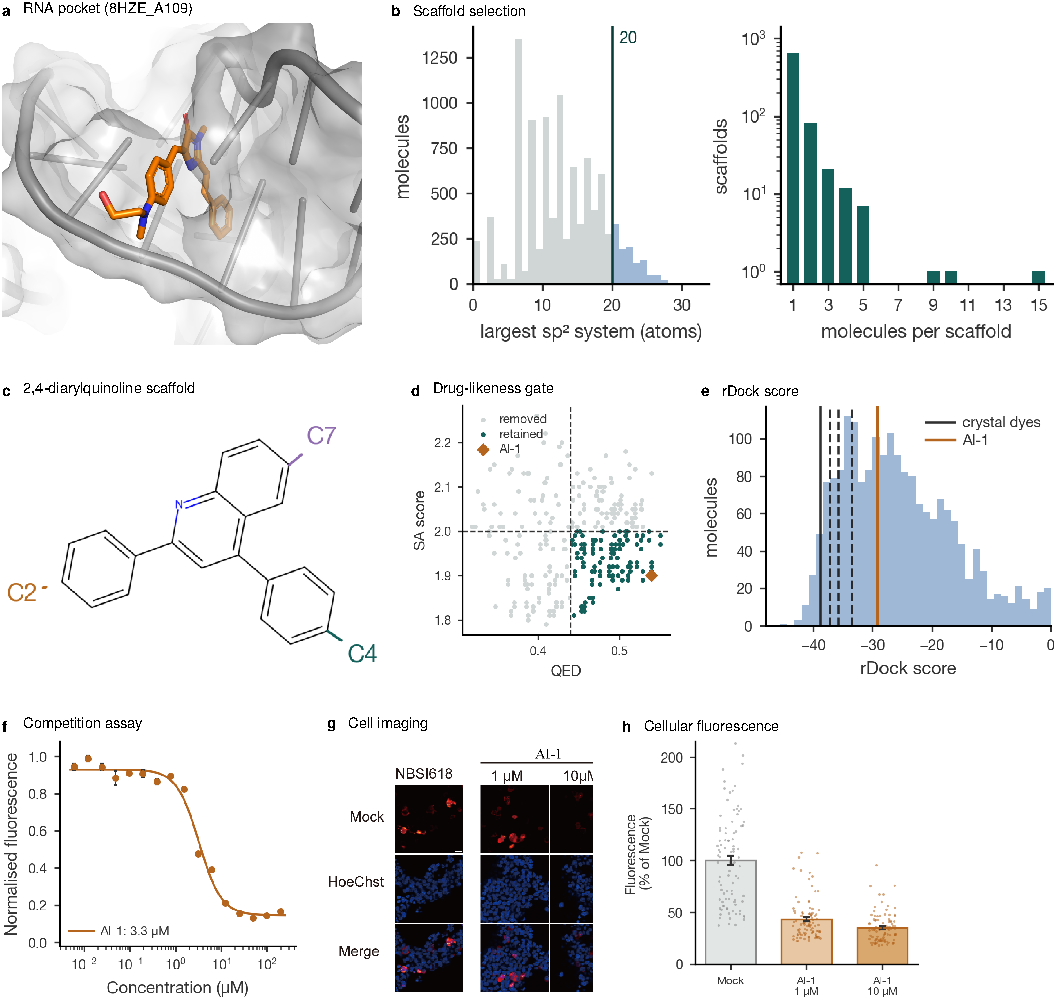
\includegraphics[width=140mm]{figures/figure5_clivia.pdf}}
\caption{Structure-based generative design of fluorogenic ligands for the Clivia aptamer. \textbf{a}, The representative pocket (8HZE\_A109) with the crystal dye NI4; RNA is shown as a cartoon with a semi-transparent molecular surface and the ligand as sticks. \textbf{b}, Scaffold selection. Left: distribution of the largest sp$^{2}$-connected system in the 9,880 closed-shell, neutral generated molecules (grey, below the 20-atom cut; blue, at or above it). Right: distribution of scaffold repetition among the retained molecules (996 molecules, 777 scaffolds); most scaffolds occur once, and the most frequent scaffold occurs 15 times. \textbf{c}, Substitution positions and substituent vocabulary. Left: the 2,4-diarylquinoline core with the three variable positions marked (C4-aryl para, C2-aryl para, quinoline C7). Right: number of molecules carrying each substituent at each position, counted over the 4,948 products that retained the intact three-ring system. \textbf{d}, Al-1 (orange) and Al-2 (purple) in the binding pocket, in the poses used for scoring. \textbf{e}, QED versus SA score for the 448 molecules (dashed lines, QED $=0.44$ and SA $=2.00$); 198 molecules are retained (teal), and Al-1 and Al-2 are marked. \textbf{f}, Distribution of the in-place-minimised rDock score across the 1,908 scored molecules of the reference enumeration; the four crystal dyes (black; NI4 $=-38.9$) and Al-1/Al-2 are marked. \textbf{g}, Competition dose--response for Al-1 and Al-2 (points, mean $\pm$ SD; lines, four-parameter logistic fits). \textbf{h}, Representative confocal images of Clivia-aptamer-expressing cells treated with Al-1 or Al-2 (NBSI618 channel, Hoechst nuclear stain, merge); Mock, untreated. \textbf{i}, Quantification of cellular fluorescence from \textbf{h} (93 cells per condition; bars, mean; error bars, SEM; dots, individual cells; percentage of the Mock mean).}
\label{clivia_case_fig}
\end{figure}

\subsection{NA2smol generation yields an experimentally validated ligand candidate for the KRAS promoter G-quadruplex}

We applied the workflow to the KRAS promoter G-quadruplex (Fig.~5a; Methods). Library expansion and multi-objective scoring narrowed the 10,077 unique molecules generated for the BER102 site to 293 Tier-1 candidates (selection rule in Methods), of which 34 had PubChem records and 14 were vendor-listed (Fig.~5b--f).

The top-ranked Tier-1 candidate, 2,2$'$-methylenebis(benzothiazole) (candidate 01 in Fig.~5f; PubChem compound identifier (CID) 74755), was obtained commercially and tested experimentally.

In a ThT competition assay (Methods) the compound reduced normalised ThT fluorescence in a concentration-dependent manner, with a four-parameter logistic fit giving a DC$_{50}$ of 22.4~$\mu$M (Fig.~5g). Generation followed by post-processing therefore narrowed the 10,077-molecule library to a set of vendor-listed candidates and prioritised one for experimental evaluation.

\begin{figure}[!htbp]
\centering
\makebox[\textwidth][c]{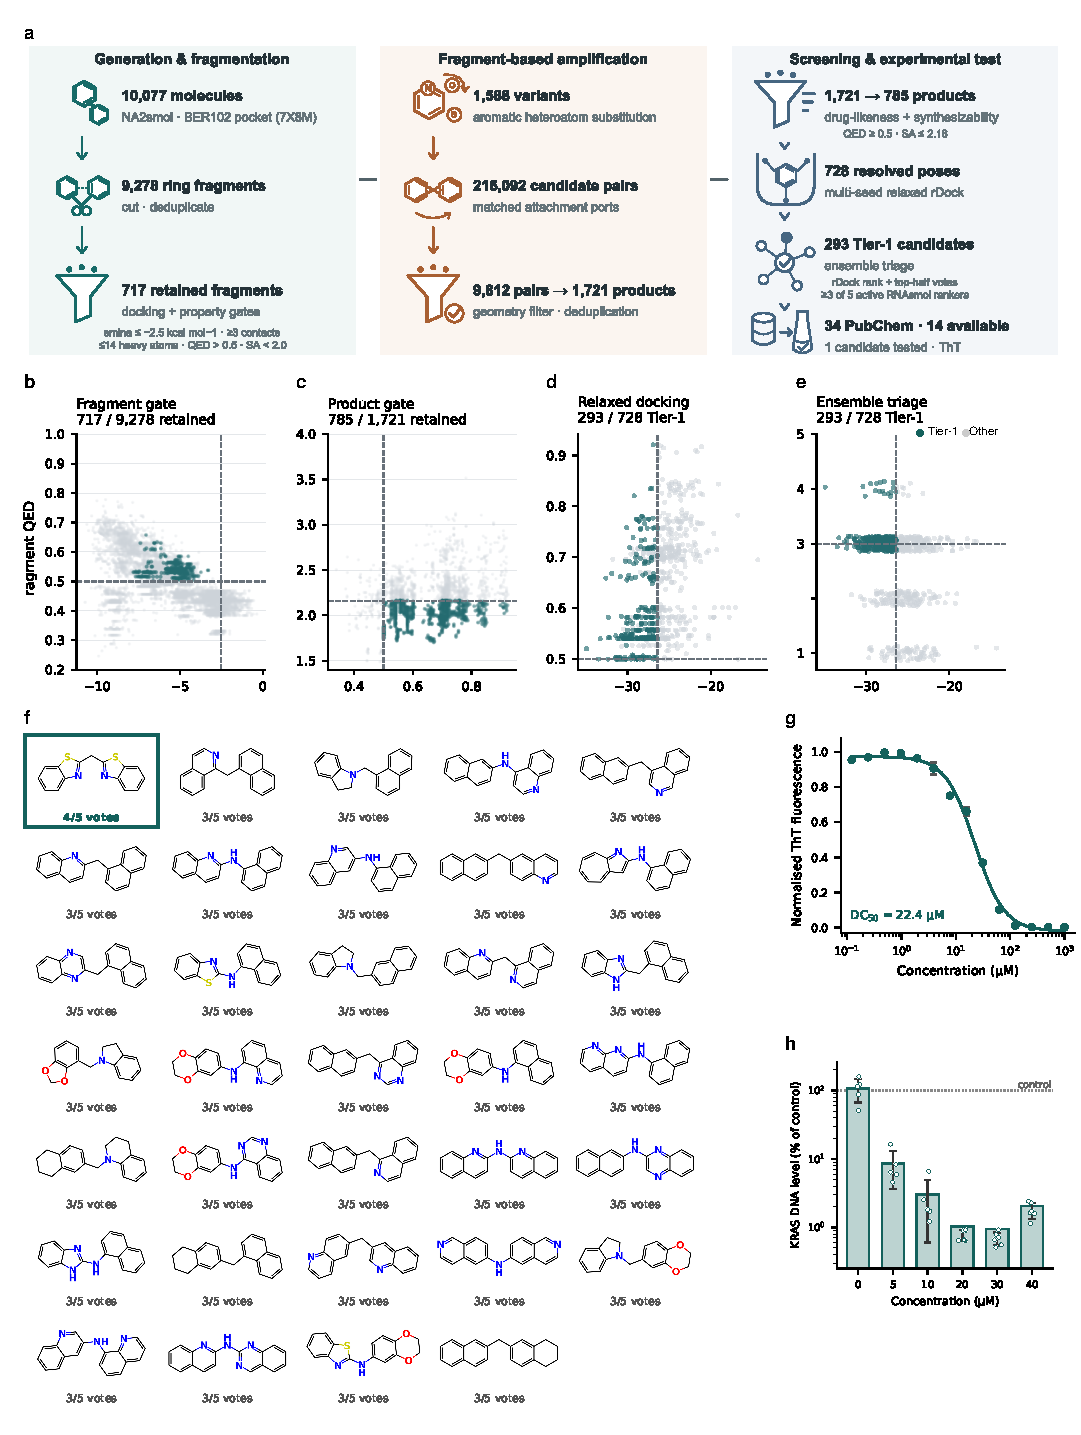
\includegraphics[width=140mm]{figures/figure5_kras.pdf}}
\caption{Experimental validation of an NA2smol-derived ligand candidate for the KRAS promoter G-quadruplex. \textbf{a}, NA2smol generation at the BER102 site (7X8M), post-processing, candidate prioritisation and experimental testing. \textbf{b}, Fragment gate: smina score versus QED across pooled ring fragments (dashed lines: $-2.5$~kcal~mol$^{-1}$ and QED $=0.5$; additional gates in Methods). \textbf{c}, Product gate: QED versus SA across assembled products (dashed lines: QED $=0.5$ and SA $=2.16$). Teal denotes retained molecules in \textbf{b},\textbf{c}. \textbf{d}, Relaxed rDock score versus QED across dock-resolved products; Tier-1 candidates are teal and others grey. Dashed lines mark the rDock median and QED $=0.5$. \textbf{e}, RNAsmol votes versus rDock score; the dashed line marks three votes and vertical jitter is used. \textbf{f}, PubChem-recorded Tier-1 candidates ordered by votes (descending), rDock (ascending) and CID, drawn at uniform bond length and labelled with their vote count out of five. The framed structure is candidate 01 (CID 74755, four votes), which was tested experimentally; the others have three votes. \textbf{g}, ThT fluorescence response for candidate 01 with a four-parameter logistic fit; points and error bars show means and SDs from three independent measurements per concentration. \textbf{h}, KRAS transcript level measured by quantitative reverse-transcription PCR on a logarithmic scale after treatment with the indicated concentrations of candidate 01, with GAPDH as internal reference (bars, mean; error bars, SD; open circles, individual replicates; $n=5$--$6$ from two independent experiments, normalised to the untreated control; dotted line, 100\% control level).}
\label{kras_case_fig}
\end{figure}



\begin{table}[!htbp]
\centering
\scriptsize
\setlength{\tabcolsep}{1.2pt}
\resizebox{\textwidth}{!}{%
\begin{tabular}{@{}lccccccccccc@{}}
\toprule
\textbf{Method} & \textbf{Dock.} & \textbf{RMSD} & \textbf{QED} & \textbf{SA} & \textbf{SEI} & \textbf{Succ.} & \textbf{p@500} & \textbf{p@200} & \textbf{Rec.} & \textbf{Spec.} & \textbf{Top-2 $\uparrow$} \\
\midrule
\multicolumn{12}{@{}l}{\textit{Fig. 2a — DUD-E protein}} \\
ED2Mol & $-6.06$ & 1.87 & \textbf{0.736} & \underline{3.04} & \textbf{0.128} & \underline{97.2\%} & \textbf{97.1\%} & \textbf{93.6\%} & \underline{0.482} & $-0.019$ & \textbf{7/10} \\\\
NA2smol & \underline{$-8.19$} & \underline{0.87} & \underline{0.647} & 3.14 & \underline{0.114} & 95.1\% & 78.7\% & 63.9\% & \textbf{0.656} & \underline{+0.019} & \underline{6/10} \\\\
Pocket2Mol & $-5.89$ & 1.47 & 0.565 & \textbf{3.00} & 0.092 & \textbf{97.4\%} & \underline{86.2\%} & 45.7\% & 0.417 & $-0.015$ & 3/10 \\\\
MolCRAFT & $\mathbf{-9.86}$ & \textbf{0.38} & 0.527 & 4.11 & 0.106 & 93.1\% & 71.1\% & 39.1\% & 0.331 & $-0.152$ & 2/10 \\\\
DiffSBDD & $-5.47$ & 2.79 & 0.493 & 5.67 & 0.057 & 81.8\% & 55.6\% & 42.6\% & 0.457 & \textbf{+0.077} & 1/10 \\\\
FLAG & $-3.86$ & 3.25 & 0.400 & 6.57 & 0.043 & 95.5\% & 84.2\% & \underline{76.7\%} & 0.142 & $-0.006$ & 1/10 \\\\
GraphBP & $-1.33$ & 4.45 & 0.481 & 6.37 & 0.014 & 29.5\% & 11.6\% & 8.2\% & 0.093 & $-0.007$ & 0/10 \\\\
\midrule
\multicolumn{12}{@{}l}{\textit{Fig. 2d — RNA test set}} \\
ED2Mol & $-5.16$ & 1.62 & \textbf{0.699} & \textbf{2.85} & \textbf{0.116} & \textbf{97.7\%} & \textbf{97.6\%} & \textbf{94.8\%} & 0.077 & \underline{+0.019} & \textbf{7/10} \\\\
NA2smol & $\mathbf{-7.27}$ & \underline{1.12} & \underline{0.641} & 3.53 & \underline{0.103} & 92.0\% & 66.6\% & 47.7\% & \textbf{0.218} & \textbf{+0.037} & \underline{6/10} \\\\
MolCRAFT & \underline{$-6.91$} & \textbf{0.39} & 0.421 & 3.84 & 0.062 & \underline{96.7\%} & 84.5\% & 66.4\% & 0.059 & $-0.012$ & 3/10 \\\\
Pocket2Mol & $-5.86$ & 1.32 & 0.554 & \underline{2.94} & 0.070 & 70.5\% & 58.9\% & 22.9\% & \underline{0.080} & $-0.076$ & 2/10 \\\\
FLAG & $-3.52$ & 3.10 & 0.377 & 6.54 & 0.044 & 95.1\% & \underline{90.1\%} & \underline{86.7\%} & 0.015 & $-0.000$ & 2/10 \\\\
DiffSBDD & $-2.95$ & 4.36 & 0.458 & 5.57 & 0.038 & 93.9\% & 79.5\% & 70.0\% & 0.080 & $-0.010$ & 0/10 \\\\
GraphBP & $-2.37$ & 4.33 & 0.460 & 6.42 & 0.045 & 35.3\% & 14.9\% & 10.7\% & 0.004 & +0.002 & 0/10 \\\\
\midrule
\multicolumn{12}{@{}l}{\textit{Fig. 3a — RNA test set, four configurations}} \\
NA2smol & $\mathbf{-7.27}$ & \underline{1.12} & \textbf{0.641} & \textbf{3.53} & \underline{0.103} & \textbf{92.0\%} & \textbf{66.6\%} & \textbf{47.7\%} & \textbf{0.218} & \textbf{+0.037} & \textbf{10/10} \\\\
Pretrain+Constrain & \underline{$-7.21$} & 1.26 & \underline{0.619} & 4.35 & \textbf{0.104} & 83.8\% & \underline{64.4\%} & \underline{37.0\%} & 0.132 & \underline{+0.030} & \underline{6/10} \\\\
Baseline & $-6.03$ & \textbf{1.09} & 0.484 & \underline{3.86} & 0.078 & \underline{91.2\%} & 58.1\% & 29.2\% & \underline{0.141} & +0.010 & 4/10 \\\\
Pretrain Only & $-7.19$ & 1.32 & 0.509 & 5.11 & 0.096 & 46.3\% & 30.2\% & 13.2\% & 0.035 & +0.008 & 0/10 \\\\
\bottomrule
\end{tabular}}
\caption{Radar-metric values for the benchmark comparison (Fig.~2a,d) and the configuration comparison (Fig.~3a). Dock., smina docking score (kcal mol$^{-1}$); RMSD (\AA) after pose relaxation; QED; SA, synthetic accessibility score; SEI, surface efficiency index ($-$docking score / TPSA); Strain, conformational strain energy (kcal mol$^{-1}$, scientific notation above 10$^3$); ECFP4 rec., the observed recovery on the ECFP4-Tanimoto axis. Values are pooled medians over all of a method's molecules. \textbf{Bold} marks the best value in each benchmark group and \underline{underline} the second best. Lower is better for Dock., RMSD and SA; higher is better for QED, SEI, Succ., p@500, p@200, Rec. and Spec. Top-2 counts, out of the ten metrics, how many the method ranks first or second on within its group; it takes the same emphasis and orders the rows. These are the single-number summaries of the distributions whose normalised retention-curve integrals are drawn in the radars; the normalised scores themselves are in Supplementary Table~12.}
\label{radar_values_tab}
\end{table}


\section{Discussion}

Transferring structure-based molecular generation to nucleic-acid binding sites requires bridging a severe training-data asymmetry without relying on residue-specific pocket encodings. By restricting pocket conditioning to descriptors shared across proteins and nucleic acids, NA2smol allows ligand-level structural priors and protein-complex supervision to inform generation in nucleic-acid pockets. The auxiliary objectives govern distinct aspects of candidate quality: pretraining alone improved docking scores at the cost of conformational plausibility, consistent with a channel in which electron density traces the envelope of a physically reasonable ligand, so a model that follows it is optimised for shape complementarity while receiving little signal on internal bond geometry. Coupling the student to the frozen teacher through output alignment and cross-view contrastive learning reconciled these requirements, preserving the docking advantage while restoring low-strain geometry.

The protein-trained baselines retained far fewer candidates than NA2smol under the common downstream pipeline. To test whether the residue assignment required to run them on RNA accounted for part of that gap, every baseline with a residue-type channel was run on DUD-E twice, once with its native protein residue types and once with every residue type reassigned at random (Extended Data Fig.~1; Extended Data Table~9); GraphBP and ED2Mol take no residue-type input. FLAG was unaffected on all eight metrics (largest $|d_z|=0.19$), MolCRAFT and Pocket2Mol moved moderately and in both directions, and DiffSBDD was sensitive, losing pose-relaxation quality, surface efficiency and ECFP4 similarity ($d_z=-1.13$, $-0.58$ and $-0.46$) and falling from 1,093 to 373 molecules at the first screening tier. The ordering follows how much pocket chemistry each encoder carries in its residue channel, from DiffSBDD's C$\alpha$-level representation to FLAG's element-level chemistry: residue identity is the aspect of a pocket that transfers least between protein and nucleic-acid chemistry.

The chemical-overlap audit showed that the full model had the largest recovery reduction under the pretraining-analogue filter, suggesting that its retrospective ECFP4 recovery is more sensitive to chemically familiar reference actives within the pretraining chemical space; method rankings persist after excluding fine-tuning analogues (Supplementary Note~5). Beyond retrospective benchmarks, two case studies connect generation to experiment. In the Clivia aptamer, the crystallographic ligands provide an internal reference: the model reproduced one scaffold more often than any other, the substituents placed at three positions defined a synthesisable combinatorial library, and two library members displaced the aptamer dye in solution and in cells. In the KRAS promoter G-quadruplex, generation was combined with post-processing and computational prioritisation, yielding a bis-benzothiazole that reduced normalised ThT fluorescence in a concentration-dependent manner.

NA2smol provides a framework for three-dimensional molecular generation in a target class for which complex structures are comparatively limited, and combining common physicochemical pocket descriptors, ligand-level structural pretraining and complementary training objectives is a practical strategy for constructing generative models for nucleic-acid pockets.

\section{Methods}

\subsection{Model architecture}

NA2smol is based on a BFN backbone \cite{graves2023bfn} and comprises three modules: a condition encoder, a ligand encoder and a ligand decoder. The condition encoder processes electron-density maps during pretraining and pocket structures during fine-tuning, while the decoder outputs atomic coordinates and types.

\subsubsection{Condition encoder}

The encoder handles two input modalities to enable cross-domain knowledge transfer.

\medskip
\noindent\textbf{Electron density encoding.} During pretraining, the cctbx library \cite{grossekunstleve2002cctbx} computes ligand electron density maps from which \(M\) points are sampled from high-density regions (\(\rho(\mathbf{r}) > \rho_0\), where \(\rho_0\) is a fixed density threshold):
\[
\mathbf{p}_i \sim \rho(\mathbf{r}) \cdot \mathbb{I}[\rho(\mathbf{r}) > \rho_0], \quad i=1,\dots,M,
\]
where \(\mathbb{I}[\cdot]\) is the indicator function. The density is represented on a discrete voxel grid, following ED2Mol \cite{ed2mol2025}, and we refer to it as electron density throughout. Each point receives a pharmacophore label \(l_i \in \{0,1,2,3\}\) based on proximity to hydrogen-bond donor (HBD) or acceptor (HBA) atoms: 0, neither; 1, HBD only; 2, HBA only; 3, both. Labels are embedded via a learnable lookup table and combined with positional encodings to form \(\mathbf{h}_{\text{ed}}\).

\medskip
\noindent\textbf{Pocket structure encoding.} During fine-tuning and inference, pockets are encoded through a shared physicochemical feature stream:
\begin{equation}
\mathcal{P} = \mathcal{P}_{\text{uni}} = \text{PocketEncoder}(\text{pharmacophore}, \text{hybridisation}, \text{vdW radius}, \text{partial charge}),
\end{equation}
where $\text{PocketEncoder}$ denotes the shared pocket encoder, projecting these shared descriptors into a latent space without residue-specific features. Stochastic feature dropout regularises the encoder. Pocket atoms are selected geometrically: a residue is retained in full when at least one of its atoms lies within 12~\AA\ of the reference ligand, so each kept residue contributes all of its atoms. Water molecules and non-nucleotide, non-amino-acid, non-ion hetero groups are excluded.

\subsubsection{Ligand representation and decoder}

Each ligand atom is represented by element type (one-hot), hybridisation state and an aromaticity flag, embedded via linear projection and combined with time embeddings. The decoder uses an equivariant graph transformer with interleaved X2H (coordinate-to-feature) and H2X (feature-to-coordinate) attention layers for coordinate prediction equivariant under three-dimensional rotations and translations (SE(3)). Edges are built as a single \(k\)-nearest-neighbour graph (\(k=32\)) over the ligand atoms together with the conditioning point cloud: pocket atoms during fine-tuning and electron-density points during pretraining. Each edge receives one of four types according to whether its source and destination atoms belong to the ligand.

\subsubsection{Training objectives}

Following the BFN formulation \cite{graves2023bfn}, the primary losses for timestep \(t \sim U(0,1)\) are:
\begin{align}
\mathcal{L}_{\text{coord}} &= -\ln(\sigma_1) \cdot \mathbb{E}_{t, p_F(\theta|\mathbf{x};t)} \bigl[ \sigma_1^{-2t} \|\hat{\mathbf{x}}(\theta,t) - \mathbf{x}\|^2 \bigr], \label{eq:coord} \\
\mathcal{L}_{\text{type}} &= K\beta_1 \cdot \mathbb{E}_{t, p_F(\theta|\mathbf{x};t)} \bigl[ t \| \mathbf{e}_{\mathbf{x}} - \hat{\mathbf{e}}(\theta,t) \|^2 \bigr], \label{eq:type}
\end{align}
with \(\sigma_1 = 0.03\), \(\beta_1 = 1.5\), \(K\) atom-type classes, \(\mathbf{e}_{\mathbf{x}}\) the one-hot true type, and \(\hat{\mathbf{e}}(\theta,t)\) the predicted type distribution.

\medskip
\noindent\textbf{Contrastive pathway.} The full model additionally applies a cross-view contrastive loss between the student and the electron-density teacher. In each path, atom representations are pooled into a molecule-level representation by attention pooling, projected through a shared projection head and $L_2$-normalised. A symmetric InfoNCE objective then treats the student and teacher representations of the same molecule as a positive pair and representations of different molecules in the batch as negatives, giving the term $L_{\mathrm{contrastive}}$. The full model therefore minimises the objective of Eq.~\eqref{eq:total}, which carries the additional $0.1L_{\mathrm{contrastive}}$ term. The alignment weight $w(t)=\mathrm{sigmoid}(10(t-0.5))$ increases monotonically with $t$, so the alignment acts most strongly as $t\to1$.

\medskip
\noindent\textbf{Teacher--student alignment loss.} The active auxiliary loss aligns the pocket-conditioned student with a frozen electron-density-conditioned teacher model of the same architecture. Both are initialised in the fine-tuning configuration from the electron-density-pretrained teacher checkpoint (step 369999), with the teacher parameters frozen throughout and only the student updated; no protein-only fine-tuning is applied to the teacher. Let \(\hat{\mathbf{x}}^{\text{ED}}, \hat{\mathbf{p}}_0^{\text{ED}}\) denote teacher predictions and \(\hat{\mathbf{x}}, \mathbf{p}_0\) student predictions. The loss combines coordinate alignment and a symmetric Kullback--Leibler (KL) divergence:
\begin{align}
\mathcal{L}_{\text{coord-align}} &= \frac{1}{N}\sum_{i=1}^{N} \|\hat{\mathbf{x}}_i^{\text{ED}} - \hat{\mathbf{x}}_i\|^2, \\
\mathcal{L}_{\text{type-align}} &= \frac{1}{2}\bigl(D_{\text{KL}}(\mathbf{p}_0 \,\|\, \hat{\mathbf{p}}_0^{\text{ED}}) + D_{\text{KL}}(\hat{\mathbf{p}}_0^{\text{ED}} \,\|\, \mathbf{p}_0)\bigr),
\end{align}
where \(D_{\text{KL}}(\mathbf{p} \,\|\, \mathbf{q}) = \sum_k p_k (\log p_k - \log q_k)\) with a \(10^{-8}\) stabiliser. The teacher and student receive the same noisy ligand state, but different conditioning inputs: ED for the teacher and the pocket for the student. The alignment compares the predicted coordinates \(\hat{\mathbf{x}}\) and the predicted atom-type distribution \(\mathbf{p}_0\). The globally averaged alignment losses are multiplied by $\mathrm{sigmoid}(10(t-0.5))$ and added to the outer training loss.

\medskip
\noindent\textbf{Training objective.} Let $w_i$ be the primary-loss weight (10 for nucleic-acid records when the batch marker is present, 1 otherwise), and let $\bar g$ be the batch mean of $\mathrm{sigmoid}(10(t-0.5))$. The fine-tuning configuration uses
\begin{equation}
\mathcal{L}_{\mathrm{total}}=\operatorname{mean}\!\left[w_i(\mathcal{L}_{\mathrm{coord},i}+\mathcal{L}_{\mathrm{type},i})\right]+0.1\bar g\left(\mathcal{L}_{\mathrm{coord-align}}+\mathcal{L}_{\mathrm{type-align}}\right)+0.1\mathcal{L}_{\mathrm{contrastive}}.
\label{eq:total}
\end{equation}
The baseline was trained with the primary Bayesian-flow losses only. Pretrain-Only fine-tunes from the pretrained weights without a teacher checkpoint, which removes the alignment loss. Pretrain+Constrain applies the alignment loss, and the full model applies both the alignment and the cross-view contrastive term; the last term of Eq.~\eqref{eq:total} is therefore present only in the full model. Supplementary Note~4 gives the forward-pass pseudocode.

\subsubsection{Sampling}

At inference, the model reverses the Bayesian flow from a prior (\(\boldsymbol{\mu}_{\text{coord}} = \mathbf{0}\), \(\boldsymbol{\theta}_{\text{type}} = \mathbf{1}/K\)) over \(N = 1000\) steps:

\begin{algorithm}[H]
\caption{NA2smol sampling}
\label{alg:sampling}
\begin{algorithmic}
\State Initialise \(\boldsymbol{\mu}_{\text{coord}}^{(0)} = \mathbf{0}\), \(\boldsymbol{\theta}_{\text{type}}^{(0)} = \mathbf{1}/K\)
\For{\(i = 1\) to \(N\)}
 \State \(t = i/N\)
 \State \(\hat{\mathbf{x}}^{(i)}, \hat{\mathbf{e}}^{(i)} = \text{Model}(\boldsymbol{\mu}_{\text{coord}}^{(i-1)}, \boldsymbol{\theta}_{\text{type}}^{(i-1)}, t, \text{condition})\)
 \State Draw the output atom-type class \(k \sim \hat{\mathbf{e}}^{(i)}\) (bookkeeping only; not fed back into the state)
 \State \(\boldsymbol{\mu}_{\text{coord}}^{(i)} \gets \gamma(t_{\text{next}}) \hat{\mathbf{x}}^{(i)} + \sqrt{\gamma(t_{\text{next}})(1-\gamma(t_{\text{next}}))}\, \boldsymbol{\epsilon}_{\text{coord}}\), with \(t_{\text{next}} = i/N\), \(\gamma(t)=1-\sigma_1^{2t}\), \(\boldsymbol{\epsilon}_{\text{coord}} \sim \mathcal{N}(\mathbf{0},\mathbf{I})\)
 \State \(\boldsymbol{\theta}_{\text{type}}^{(i)} \gets \mathrm{softmax}\bigl(\beta_1 t_{\text{next}}^2 (K \hat{\mathbf{e}}^{(i)} - \mathbf{1}) + \sqrt{\beta_1 t_{\text{next}}^2 K}\, \boldsymbol{\epsilon}_{\text{type}}\bigr)\), with \(\boldsymbol{\epsilon}_{\text{type}} \sim \mathcal{N}(\mathbf{0},\mathbf{I})\)
\EndFor
\State \(\hat{\mathbf{x}}_{\text{final}}, \hat{\mathbf{e}}_{\text{final}} = \text{Model}(\boldsymbol{\mu}_{\text{coord}}^{(N)}, \boldsymbol{\theta}_{\text{type}}^{(N)}, t=1, \text{condition})\)
\State \Return \(\hat{\mathbf{x}}_{\text{final}}, \hat{\mathbf{e}}_{\text{final}}\)
\end{algorithmic}
\end{algorithm}

Algorithm~\ref{alg:sampling} describes the sampling strategy used for the reported results. Each state is refreshed in closed form from the model's own predictions \((\hat{\mathbf{x}}^{(i)}, \hat{\mathbf{e}}^{(i)})\) evaluated at the next time step \(t_{\text{next}}=i/N\). Run-to-run variability enters through the Gaussian draws \(\boldsymbol{\epsilon}_{\text{coord}}\) and \(\boldsymbol{\epsilon}_{\text{type}}\) at each step, through the random seed, and, in the unconstrained path, through the ligand-size draw described below. All benchmark results use unconstrained generation from the target pocket.

The number of ligand heavy atoms \(n_{\text{heavy}}\) is set before sampling. For the RNA test-set and DUD-E benchmark generations, \(n_{\text{heavy}}\) is drawn from a piecewise-Gaussian size model. Specifically, the cavity volume of the conditioning pocket selects a bin in a table of per-bin means and standard deviations compiled from the heavy-atom counts of ligands in PDB structures (RNA and protein tables compiled separately). The value \(n_{\text{heavy}}\) is then drawn from that Gaussian and clamped to the interval of 1.5 standard deviations around the bin mean. The same table is used during training and generation, so generated sizes follow the empirical heavy-atom distribution of the training ligands.

\subsubsection{Clivia aptamer case study: pockets, enumeration, scoring and assays}

\textbf{Pocket definition.} Dye-defined pockets were extracted around each crystallographically independent Clivia dye in 8HZD, 8HZE, 8HZF, 8HZJ, 8HZK, 8HZL and 8HZM; all nucleotides with any atom within 14~\AA\ of the ligand were retained, and pockets were superposed on nucleotide C4$'$ and phosphate atoms.

\textbf{Scaffold selection.} The 10,000 molecules generated for the 8HZE\_A109 pocket (100 sampling steps) were filtered with hard criteria: closed-shell and neutral; largest sp$^{2}$-connected component $\geq 20$ atoms (the value measured for each of the four Clivia crystal dyes NI4, O2I, NJL and O00); at least two aromatic rings; SA score $\leq 4$; molar mass 250--600~Da; TPSA $\leq 120$~\AA$^{2}$; at most nine rotatable bonds. Bemis--Murcko scaffolds were then counted among the retained molecules and ranked by repetition; the most frequent scaffold was taken as the design core.

\textbf{Inpainting and enumeration.} The ring atoms of the 2,4-diarylquinoline core were held fixed and the substituents were generated with the inpainting model (100 sampling steps). Substituent identity at the three variable positions was assigned by quinoline-anchored site identification and a rule-based classifier over the 4,948 products that retained the intact three-ring system. Every substituent observed at least once at a position was admitted to the combinatorial enumeration, giving 448 molecules.

\textbf{Non-docked scoring.} Molecules were minimised in place with the rDock nucleic-acid scoring function under a rigid receptor, with the receptor MOL2 rebuilt with a per-residue SUBSTRUCTURE section, and scored with the same scoring function. The four Clivia crystal dyes were scored from their crystallographic coordinates after superposition onto the 8HZE pocket (pocket RMSD 0.42--0.56~\AA). Candidates were filtered by QED $\geq 0.44$ and SA score $\leq 2.00$ and ordered by the equal-weight mean of the percentile ranks of the minimised rDock score and the SA score.

\textbf{Competition assays.} Four-parameter logistic fits were computed for Al-1 ($n=16$ wells) and Al-2 ($n=14$ wells). For fluorescence displacement assays, small aliquots of a stock solution of candidate 01, Al-1 or Al-2 were added to a solution containing ThT (200~nM) and the KRAS G-quadruplex (100~nM), or NBSI618 (200~nM) and the Clivia aptamer (100~nM). The final compound concentration varied from 0.0 to 20~$\mu$M. Fluorescence changes were recorded at excitation/emission wavelengths of 425/490~nm for the ThT--KRAS complex and of 510/618~nm for the NBSI618--Clivia complex, and the half-maximal displacement concentration (DC$_{50}$) was obtained by fitting the displacement data in GraphPad Prism~9.

\textbf{RNA imaging.} To validate the effects of Al-1 and Al-2 in living cells, a plasmid expressing Clivia was transfected into HEK293T cells. Cells were co-incubated with Hoechst~33342 (1~$\mu$g~ml$^{-1}$) and NBSI~618 (0.1~$\mu$M); after 20~min, Al-1 or Al-2 was added at 1~$\mu$M or 10~$\mu$M. A 561~nm laser was used and the change in fluorescence intensity at 640~nm was recorded. All imaging was performed on an Olympus SpinSR10 spinning-disk confocal microscope with a live-cell module (37~$^\circ$C, 5\% CO$_2$), a 20$\times$ objective and a Photometrics Prime BSI camera. Images were processed in Fiji, cell brightness was quantified in Fiji and statistics were computed in GraphPad Prism; 93 cells were quantified per condition from a single representative experiment, bars show the mean and error bars the SEM, and comparisons against the untreated control used Welch $t$-tests with Holm correction.

\textbf{Quantitative RT-PCR.} A549 cells were plated in 6-well plates (2~$\times$~10$^{5}$ cells per well) and allowed to adhere for 24~h, then treated with candidate 01 at the indicated concentrations for 8~h. Total RNA was isolated with an RNA extraction kit (TransGen Biotech, China) following the manufacturer's instructions, quantified by UV--Vis spectrophotometry (NanoDrop One, Thermo) and reverse-transcribed into complementary DNA with the HiScript~Q RT SuperMix kit (Vazyme Biotech, China). Quantitative RT-PCR was performed on a LightCycler~480~II system (Roche, Germany) with SYBR Green detection, and target gene expression was normalised to GAPDH as the endogenous reference. All reactions were run in triplicate across three independent biological replicates.

\subsubsection{Post-processing for the KRAS G-quadruplex case study}

The KRAS G-quadruplex case study (Fig.~5) produced a molecular library from the BER102 site of the KRAS promoter G-quadruplex (PDB 7X8M) with the fine-tuned NA2smol checkpoint. Four independent sampling streams produced 10,077 unique molecules. The post-processing workflow proceeded in two phases.

\medskip
\noindent\textbf{Library-expansion phase.} Each generated molecule was decomposed into ring fragments by fragment cutting followed by removal of duplicates, yielding 9,278 unique fragments. A fragment entered the pool if it satisfied smina $\leq -2.5$~kcal~mol$^{-1}$, QED $> 0.5$ and SA score $< 2.0$, with at least three interacting atoms and at most 14 heavy atoms; this filter retained 717 pooled fragments. In these pooled fragments, we enumerated atom substitutions at degree-two aromatic heteroatom positions in five- or six-membered rings (replacing N, O or S with N, O, S or C, subject to valence checks), producing 1,588 variants. Each variant was then scored by rDock \cite{ruizcarmona2014rdock} on the BER102 system. Variants were paired by matching attachment sites. Each site records a fragment atom and the element and original position of its neighbouring atom removed during cutting. Pairs with matching removed-atom elements and positions separated by $\leq1.0$~\AA\ were joined by adding a bridging atom of that element at the midpoint. Of 216,092 candidate fragment pairs, 9,812 passed the assembly-geometry checks and yielded 1,721 unique products after removal of duplicates.

\medskip
\noindent\textbf{Scoring and selection phase.} Products passed a drug-likeness and synthesizability filter (QED $\geq 0.5$, SA score $\leq 2.16$, the median SA score in the product pool), retaining 785. Each was relaxed in the BER102 pocket by multi-seed minimise-in-place docking (three seeds, five runs per seed; the lowest-intermolecular-energy pose within 2.0~\AA\ RMSD was kept), resolving 728 molecules. The RNAsmol interaction-scoring ensemble \cite{ma2025rnasmol} comprises six sub-models; sub-models whose binder-probability scores were constant across the candidate set (standard deviation $\leq 10^{-6}$) were dropped, leaving five active rankers. Each active ranker ranked the candidates by its binder probability, and a candidate earned a vote when its rank fell in the top half of the resolved set. A product was assigned to Tier-1 when it earned votes from at least $\lfloor k/2\rfloor+1$ of the $k=5$ active rankers ($\geq3$ of $5$) and fell in the upper half of the relaxed rDock ranking. This rule selected 293 candidates, which were queried against PubChem for registration and purchasability.

\medskip
\noindent\textbf{Experimental validation.} The Tier-1 molecule 2,2$'$-methylenebis(benzothiazole) (PubChem CID 74755) was obtained commercially and tested in the ThT fluorescence competition assay described below.

\subsection{Data preparation}

For pretraining, we curated a dataset of approximately 2.4 million molecules from the ZINC database \cite{irwin2020zinc20} and ChEMBL \cite{zdrazil2024chembl}. Two-dimensional ligand structures were converted to three-dimensional conformations using the Experimental-Torsion Knowledge Distance Geometry (ETKDG) algorithm \cite{riniker2015etkdg} in RDKit \cite{landrum2024rdkit}. These conformations were then energy-minimised with the Merck molecular force field 94 (MMFF94) \cite{halgren1996mmff}, retaining one lowest-energy conformer per molecule. From each minimised conformer, we computed simulated electron-density maps by Fourier transformation of atom-based structure factors using the cctbx crystallography toolbox \cite{grossekunstleve2002cctbx} at a target resolution of 3.5~\AA\ on a cubic grid (unit cell 50$\times$50$\times$50~\AA, space group $P1$). This follows the electron-density-based pretraining procedure introduced in ED2Mol \cite{ed2mol2025}. High-density grid points ($\rho(\mathbf{r}) > \rho_0$) were then sampled (499 points per molecule at the standard resolution; 999 at the fallback resolution). They were labelled with hydrogen-bond donor/acceptor pharmacophore types to form the point-cloud conditioning input used during the unsupervised pretraining stage. Protein--ligand structures were drawn from two sources: experimentally determined structures from the Protein Data Bank (PDB) \cite{berman2000pdb} and docked poses from CrossDocked2020 \cite{francoeur2020crossdocked}. Protein pockets too similar to the DUD-E test pockets were removed by the shape- and ICP-based filter described below. Together with the nucleic-acid records, this gave 126,899 protein--ligand training structures and 738 nucleic-acid--ligand records (Extended Data Table~5).

The curated nucleic-acid record set contains 738 records, partitioned into 356 training and 382 validation records that share no record index. A structure-identifier cross-check against the 27 evaluable RNA systems finds two training identifiers (1yrj and 2o3x) and eleven validation identifiers; the benchmark split is defined at the record level. The preprocessing maps nucleic-acid residue names to generic nucleotide labels. The 738 nucleic-acid records comprise 457 RNA, 274 DNA and 7 hybrid entries by RCSB polymer annotation (Supplementary Table~4). For the protein training set, structural overlap with the DUD-E test pockets was controlled by a two-stage filtering pipeline. Pocket structures were first pre-filtered with a 12-dimensional pocket-shape descriptor comprising the mean, standard deviation, skewness and kurtosis of distances to the centroid, pairwise distances and sampled triangle areas. Surviving candidates were then refined by Iterative Closest Point (ICP) with Kabsch alignment (RMSD threshold 2.0~\AA). Protein pockets whose ICP RMSD to any DUD-E test pocket fell below this threshold were excluded from the training set. Pocket structures were processed to extract atomic coordinates and transferable physicochemical descriptors. Pharmacophore labels (hydrogen-bond donor/acceptor types) were assigned with the RDKit feature factory \cite{landrum2024rdkit}, and hybridisation states were read from the molecular graph. Van der Waals radii were taken from the element table, and partial charges were estimated with the Gasteiger method in RDKit. Ligand molecules were standardised using RDKit \cite{landrum2024rdkit} to obtain consistent atom typing and bond orders.

\subsection{Training details}

NA2smol is implemented using PyTorch \cite{paszke2019pytorch} and PyTorch Geometric (PyG) \cite{fey2019pyg}. RDKit \cite{landrum2024rdkit} and PyMOL \cite{pymol2024} are used for molecular structure processing and visualisation. The model configuration uses a hidden dimension of 128, one block of nine attention layers and 16 attention heads. The full configuration is provided in Extended Data Table~1.

The ligand-only electron-density pretraining uses the same Bayesian-flow objective together with a self-supervised contrastive term. Two views of one ligand state are formed by perturbing the flow time ($t_{\mathrm{aug}}=t+0.1\,\epsilon$, $\epsilon\sim\mathcal{N}(0,1)$, clipped to the admissible range). A symmetric InfoNCE objective then pulls the representations of adjacent flow states together while pushing those of different molecules apart (the two latent-space distances drawn in Fig.~\ref{overview}). The fine-tuning configuration uses the Muon optimiser \cite{bernstein2024modular} with learning rate $10^{-5}$ and weight decay 0.01. It defines a linear warmup over 4,900 steps, followed by a validation-loss plateau scheduler (factor 0.8, patience 50, minimum learning rate $10^{-6}$). Gradient clipping uses a maximum norm of 8.0.

The fine-tuning configuration uses seed 1234, a fixed batch size of 20 and alignment weights of 0.1. The electron-density teacher was initialised from step 369999, and the evaluated checkpoint for the full model is identified by step 111429; Supplementary Note~4 gives the forward-pass specification.

\subsubsection{Molecule reconstruction}

Generated atom clouds are converted to molecular graphs by inferring bonds from interatomic distances, perceiving bond orders and then sanitising the result. Bond perception first rebuilds the atom cloud as an OpenBabel molecule in which every atom is temporarily treated as carbon, setting initial connectivity by uniform covalent radii. A bond is then created between any pair of atoms whose distance is below $1.3$ times the sum of their OpenBabel covalent radii. Per-atom maximum valences are capped at the smaller of the OpenBabel and RDKit defaults, with a sulfone exception for sulfur bearing two or more oxygen neighbours. Bonds between two atoms whose maximum valence is one are deleted. Polar hydrogens are added and bond orders are perceived by OpenBabel. The original element types are then restored, formal charges on heteroatoms are adjusted from the perceived valences, and the molecule is neutralised or rejected. Molecules failing valence or RDKit sanitisation checks are discarded. Valid molecules are canonicalised and processed through the same docking and property-calculation pipeline for all methods. A target was considered evaluable for a method if at least one generated molecule remained after sanitisation and removal of molecules with non-negative docking scores. This criterion yielded the 27 shared evaluable targets of the RNA test set used in all paired analyses. The 37 RNA systems thus reduce to 27 evaluable targets shared across methods; DUD-E output coverage is method-specific (85--102 targets, depending on the source and validity criteria). Molecule-level summaries (the property, geometry and retention-curve distributions behind the radar-chart and rank-grid panels, and the yield denominators) are computed over every valid generation from all 37 systems, whereas target-level counts and paired tests use the 27 evaluable targets. The retained-molecule count of 239 is summed over the 27 evaluable targets, and its yield denominator of 35,358 is the molecule-level pool over all 37 systems (0.68\%). Figure~2b and the DUD-E ECFP4 metric axis use the fixed 101-target reference universe, counting targets without output as unrecovered. Figure~2c reports absolute screening-retention counts over method-specific outputs, without requiring reference actives. For the DUD-E sensitivity analysis, all 101 reference targets are included; a method with no valid generated molecule on a target scores zero recovery for that target. The fine-tuning-analogue filter leaves 101 targets, and the pretraining-analogue filter leaves 98 because three targets lose all their reference actives.

\subsection{Evaluation}

NA2smol is evaluated across four categories of metrics: drug-like properties, conformational validity, docking and minimisation compatibility, and bioactive molecule recovery.

\subsubsection{External generators}

The six external generators were evaluated with their public protein-oriented checkpoints and default or officially documented sampling settings under the same downstream docking, filtering and evaluation pipeline as NA2smol. Each differs in how it conditions on the pocket and in how it produces a molecule. \textbf{MolCRAFT} generates ligand coordinates with a Bayesian flow network and conditions on pocket atoms together with their amino-acid residue types. \textbf{Pocket2Mol} generates atoms and bonds autoregressively inside the pocket, also using residue-type pocket features. \textbf{ED2Mol} runs fragment-level diffusion conditioned on an electron-density map of the ligand and takes no residue-type input. \textbf{DiffSBDD} is an SE(3)-equivariant diffusion model that places ligand atoms directly in the pocket from a C$\alpha$-level pocket representation. \textbf{GraphBP} is an autoregressive normalising flow that grows the molecule atom by atom, placing each atom in a local reference frame defined by three nearby pocket atoms; its pocket vocabulary is elemental and contains no residue identity. \textbf{FLAG} is a fragment-based autoregressive model that assembles the molecule from a learned motif vocabulary conditioned on the pocket.

Four of the six therefore accept a residue-type channel (MolCRAFT, Pocket2Mol, DiffSBDD and FLAG), which has no nucleotide equivalent. For the RNA test set, each nucleic-acid residue was therefore assigned one of the 20 amino-acid residue types pseudo-randomly before inference, with the assignment fixed for the whole benchmark and atomic coordinates left unchanged. DiffSBDD requires one C$\alpha$ per residue, so a C$\alpha$ position was taken from the C1$'$ atom where a nucleotide residue had none. The effect of this assignment on the metrics is quantified separately for each residue-channel baseline in the Discussion and Extended Data Table~9. For ED2Mol, electron-density conditioning was used as implemented in its public release.

\subsubsection{Drug-like properties}

Basic drug-likeness is assessed with the QED \cite{bickerton2012qed} and SA \cite{ertl2009sa} scores, both computed with RDKit \cite{landrum2024rdkit}.

\subsubsection{Conformational validity}

PoseCheck \cite{harris2023posecheck} is used to compute the \textbf{strain energy} of each generated conformation, defined as the energy difference between the generated geometry and a local minimum conformation optimised with a molecular mechanics force field. Lower strain energies indicate conformations that are closer to local molecular-mechanics minima. Strain is computed on the same smina-minimised pose used for every other molecule-level metric, with docking and local minimisation preceding property calculation throughout. A molecule is classed as failing the strain criterion if its strain energy could not be computed within a 30~s budget or if the computed value exceeds $10^{4}$~kcal~mol$^{-1}$, and failed molecules are retained in the denominator. Both the censored median strain (Table~1) and the fraction of a method's molecules whose computed strain is at or below 200~kcal~mol$^{-1}$ (Extended Data Table~8) are tabulated. The strain axis is the corresponding retention-curve integral over $\log_{10}$ strain from 10 to $10^{4}$~kcal~mol$^{-1}$, with the same treatment of failures. As a calibration reference, the 37 crystallographic ligands of the RNA test-set pockets run through the identical protocol give a median strain of 49~kcal~mol$^{-1}$ and a 95th percentile of 746~kcal~mol$^{-1}$ (Extended Data Table~4), with 81\% of these experimentally determined poses falling at or below the 200~kcal~mol$^{-1}$ criterion.

\subsubsection{Docking and minimisation compatibility}

Rigid-receptor docking uses smina \cite{koes2013smina} (AutoDock Vina fork \cite{trott2010vina}) with default parameters. The minimise-in-place protocol locally optimises each ligand pose within the fixed receptor, yielding a docking score (kcal~mol$^{-1}$) and pose-relaxation RMSD (displacement from the locally minimised pose, used as a minimisation-stability metric). Two normalised efficiency metrics are reported, using topological polar surface area (TPSA) and the logarithm of the octanol--water partition coefficient (logP):
\begin{align}
\text{SEI} &= -\text{Docking score} \,/\, \text{TPSA}, \\
\text{LLE} &= -\text{Docking score} - \text{logP},
\end{align}
with SEI reported in kcal~mol$^{-1}$ per \AA$^{2}$; the sign conventions of both quantities rely on docking scores being negative.

\subsubsection{Bioactive molecule recovery}

Bioactive molecule recovery is assessed by fingerprint-based similarity to known active ligands.

\medskip
\noindent\textbf{ECFP4 Tanimoto similarity.} For each generated molecule $j$, the Tanimoto similarity between its ECFP4 fingerprint (radius 2, 2048 bits) \cite{rogers2010ecfp} and the reference bioactive molecules of the target is computed, and the maximum over reference molecules is retained. This continuous maximum-similarity value is also summarised by per-target medians, but the primary reference-recovery statistic of ECFP4 Tanimoto similarity (ECFP4-TS) is defined at target level, as follows.

\medskip
\noindent\textbf{Target recovery.} Recovery is evaluated on a fixed similarity window, $[l,u]=[0.25,0.50]$. For target $i$ with reference active set $A_i$, let $s_{ij}=\max_{a\in A_i}\mathrm{Tanimoto}(\mathrm{ECFP4}_j,\mathrm{ECFP4}_a)$ be the best similarity reached by generated molecule $j$. The recovery curve of the target is
\begin{equation}
R_i(\tau)=\mathbb{I}\!\left[\max_j s_{ij}\ge\tau\right], \qquad \tau\in[l,u],
\label{eq:recovery_curve}
\end{equation}
and the target's recovery is the mean of this curve over the window,
\begin{equation}
r_i=\frac{1}{u-l}\int_l^u R_i(\tau)\,d\tau .
\label{eq:recovery}
\end{equation}
The recovery of a method is $\bar r=|T|^{-1}\sum_{i\in T}r_i$ over a fixed target universe $T$, with $r_i=0$ for a target on which the method produced no valid molecule. The universe is the 101 DUD-E targets with reference actives and the 27 shared evaluable RNA targets, with fixed bounds $l$ and $u$.

The curves in Fig.~2b,e are drawn over $\tau=0.20$--$0.50$, and every recovery value reported in the text, tables and figures integrates the fixed window $[0.25,0.50]$. Molecule-level thresholded totals are also reported.

\subsubsection{Statistical summaries}

Unless otherwise stated, molecule-level metrics are first summarised as medians within each target and then aggregated across targets. Paired comparisons use the intersection of targets shared by the two methods being compared. Yield percentages are computed as the retained molecule count divided by the total number of valid generated molecules pooled across all 37 RNA systems (or all evaluated targets on DUD-E). A valid generated molecule is one that passes RDKit sanitisation and docks with a negative score. The four-tier screening cascade comprises four successive gates: Pharma.\ (docking score $<-8$~kcal~mol$^{-1}$, QED $>0.5$, SA $<5$), +SEI (Pharma.\ with SEI $>0.1$), Strict (docking score $<-9$~kcal~mol$^{-1}$, QED $>0.5$, SA $<5$, SEI $>0.15$) and a final tier. The final tier additionally requires QED $>0.6$, SA $<4$, SEI $>0.2$ and conformational strain $<200$~kcal~mol$^{-1}$. Two-sided Wilcoxon signed-rank tests are used for paired target-level comparisons. Configuration $P$ values are per-metric tests on the shared evaluable targets of the two configurations compared.

\subsubsection{Metric normalisation}

Figs.~2a,d and 3a summarise the same seven normalised metric scores per method in two visual forms. Fig.~3a displays them as a radar chart in which the radial coordinate of metric $m$ is $r_m = 1 + 2 s_m$, mapping $s_m=0$ to the inner ring ($r=1$) and $s_m=1$ to the outer ring ($r=3$). By contrast, Figs.~2a,d display them as rank grids (bubble charts) in which rows represent methods and columns represent metrics. Both the area and the shade of each mark encode that method's rank on the corresponding axis across the compared methods. The two forms carry the same underlying $s_m$: the radar states its magnitude directly, whereas the grid avoids drawing seven methods as overlapping polygons. In both cases, $s_m \in [0,1]$ is a direction-corrected normalised score defined so that a larger value always means better performance; methods that coincide on an axis have indistinguishable scores on that metric. The seven axes are computed as follows. The six property-retention axes pool molecules, whereas the ECFP4 axis weights targets equally. Paired statistical tests instead use per-target summaries, and the funnel reports absolute molecule counts and target coverage.

\medskip
\noindent\textbf{Docking score, RMSD, QED, SA score, SEI and strain energy.} $s_m$ is the normalised integral of the molecule-retention curve over the metric's threshold range $[l,u]$. For each threshold $t\in[l,u]$, the curve $R(t)$ is the fraction of the method's molecules that pass the filter at that threshold. Specifically, $R(t)=P(\text{value}\le t)$ for lower-is-better metrics (docking score, RMSD, SA score, strain) and $R(t)=P(\text{value}\ge t)$ for higher-is-better metrics (QED, SEI). The score is $s_m=\frac{1}{u-l}\int_l^u R(t)\,dt$, that is, the mean retained fraction over the threshold range, which already lies in $[0,1]$. Strain energy is evaluated on a $\log_{10}$ scale. The threshold ranges are: docking score $[-11,-3]$~kcal~mol$^{-1}$; RMSD $[0,3]$~\AA; QED $[0,1]$; SA score $[1,7]$; SEI $[0,0.3]$; and $\log_{10}$ strain over $[1,4]$ (10 to $10^{4}$~kcal~mol$^{-1}$). Molecules above that bound or without a computed strain energy contribute $R(t)=0$ at every threshold and therefore remain in the denominator. Raw metric values for every method in Figs.~2a,d and 3a are listed in Table~1, with the best and second-best values in each benchmark group marked. The corresponding normalised scores are given in Extended Data Table~8. These six axes are computed in absolute units and are directly comparable across the figures.

\medskip
\noindent\textbf{ECFP4 recovery.} The ECFP4 axis is the observed recovery itself, defined once by Eqs.~(9)--(10). That quantity already lies in $[0,1]$, so it is used as $s_m$ without further rescaling. It is deliberately not normalised across methods: normalising by each method's own permutation null gives a score that depends on that method's molecule count and target mix as well as on its recovery, and on this benchmark such normalisation drives several methods to zero for that reason rather than for a difference in performance. The permutation null, which shuffles molecule-to-target labels (1,000 permutations) and recomputes similarity against the newly assigned target's actives, is therefore used only in the supplementary analysis of target specificity (Supplementary Note~6). Both observed and null recovery use the fixed 101-target (DUD-E) and 27-target (RNA) universes.

\subsection{Chemical-overlap audit}\label{overlap_audit_methods}

Evaluation active ligands from the RNA test set and DUD-E were standardised with RDKit 2024.09.6 and represented as canonical isomeric SMILES. A parent representation (largest fragment, charges neutralised) and non-chiral Bemis--Murcko scaffolds were also derived. For every reference active, we computed exact identity, parent identity, scaffold overlap and the maximum ECFP4-Tanimoto similarity (Morgan radius 2, 2048 bits, no chirality). Each active was compared against the fine-tuning partitions (train, validation, unused and DUD-E-dropped records) and the ligand-only pretraining library (2,287,199 unique canonical SMILES). Fine-tuning and pretraining overlap were reported separately because the pretraining library contains ligand structures without target-pocket labels. For generated molecules, exact-identity overlap and fine-tuning similarity were computed over all available unique generated molecules (613,286 across both benchmarks). By contrast, similarity to the 2,287,199-molecule pretraining library was estimated from a stratified sample of approximately 4,000 unique generated molecules per benchmark and method (sample sizes and Wilson intervals in Supplementary Table~5). The same audit was extended to the molecules that survive the screening cascade, whose Bemis--Murcko scaffolds were matched against the fine-tuning and pretraining scaffolds (Supplementary Table~3).

\subsection{Recovery sensitivity analysis}\label{recovery_sensitivity_methods}

The sensitivity analyses of Fig.~3g and Extended Data Tables~6 and~7 use the recovery defined by Eqs.~(9)--(10) throughout; they differ only in which targets and reference actives are scored, never in the similarity window or in the treatment of missing output. In separate analyses, we excluded reference actives with exact matches to the fine-tuning training set, or with maximum similarity above a specified threshold (0.5, 0.6 or 0.7) to the fine-tuning training set or the pretraining library. For each filter, filtered and unfiltered recovery were recomputed on the \emph{same} eligible-target subset (targets retaining at least one reference active after filtering and present for every compared configuration). This design separates the reference-chemistry effect from the target-composition effect. Filtering removes reference actives only and does not remove generated molecules or retrain models.

\subsection{ThT fluorescence competition assays}

ThT fluorescence competition was used to measure whether candidate molecules displace pre-bound ThT from structured nucleic-acid targets. Fluorescence was measured on a Fluoromax-4 spectrofluorometer (HORIBA), using a quartz cuvette with a 10~$\times$~10~mm path length; spectra were recorded at 5~nm excitation and emission slit widths unless otherwise specified. Unless otherwise noted, chemical reagents and solvents were purchased from Sigma-Aldrich GmbH and used without further purification.

The tested compound, bis(benzo[$d$]thiazol-2-yl)methane (2,2$'$-methylenebis(benzothiazole), PubChem CID~74755), was purchased from Meck Company (cat.\ no.\ BDPH9BCD844A) after structural verification and used without further purification.

Oligonucleotides were HPLC-purified and purchased from Sangon Biotech (Shanghai, China); the KRAS promoter G-quadruplex and the qRT-PCR primers are listed in Supplementary Table~6. Stock solutions were prepared by dissolving the oligonucleotides directly into 10~mM Tris--HCl buffer (100~mM KCl, pH~7.4) and were annealed in a 90~$^\circ$C water bath for 5~min followed by slow cooling to 4~$^\circ$C. Three independent measurements were taken at each concentration, and buffer-only and buffer-plus-dye controls were included in every run.

\subsection{Limitations and scope}

The RNA test set contains 37 RNA systems, of which 27 passed validity filtering (exclusions in the per-target tables). All docking-derived scores (docking score, SEI and LLE) use rigid-receptor smina scoring, which is parameterised on protein--ligand complexes and omits nucleic-acid flexibility, metal ions, explicit water, and protonation and tautomer states. The reported RMSD measures pose relaxation during local minimisation. The training and validation records share structure identifiers with 13 benchmark systems, so the benchmark split is defined at the record level (Supplementary Table~2). The protein-trained baselines were evaluated with their published checkpoints without fine-tuning on the 738 nucleic-acid--ligand complexes, and ligand-scoring methods such as RNAmigos2 \cite{rnamigos2025} do not generate molecules. The chemical-overlap audit quantifies overlap between evaluation actives, the training and pretraining ligand sets, and generated molecules, and measures recovery after removing overlapping references, with pretraining-library similarity for generated molecules estimated from a stratified sample. ECFP4-TS measures chemical similarity to known actives. Finally, the experimental component is a single DNA G-quadruplex ThT-displacement case study without a compound-only fluorescence control, orthogonal binding assay, or measurements of affinity, selectivity or binding mode.

\section*{Data availability}

The study uses public resources including ZINC, ChEMBL, CrossDocked2020, the Protein Data Bank, the RNA test set, DUD-E, PubChem and BindingDB, as described in Methods. The code repository at \url{https://github.com/Gallo13th/NA2mol} (commit \texttt{5bd3a6b}) provides processed benchmark inputs, generated-molecule tables with per-target statistics and random seeds, and virtual-screening summaries. It also provides figure source data and the raw thioflavin T fluorescence measurements. Data tables will be released under CC BY 4.0.

\section*{Code availability}

Source code for model training, generation, evaluation, virtual-screening analysis and figure reproduction is available in \url{https://github.com/Gallo13th/NA2mol}. Large training databases, model checkpoints and generated-output archives will be deposited alongside the published version.

\section*{Acknowledgements}

Funder and computational-platform acknowledgements will be added before publication.

\section*{Author contributions}

Author contributions will be listed once the author order is finalised.

\section*{Competing interests}

The authors declare no competing interests.


\bibliography{sn-bibliography}

\newpage

\end{document}
